\chapter{Le immagini digitali}
\section{Definizione di immagine}
Useremo il Teorema del campionamento per applicarlo al concetto di immagine.
\begin{definition}
    Un'immagine è una rappresentazione grafica di valori numerici.
\end{definition}
In dettaglio un'immagine è una funzione bi-dimensionale $f(x,y)$, dove le
variabili (spaziali) $x$ e $y$ sono valori reali che definiscono la posizione
dei punti nell'immagine e $f(x,y)$ e in genere un valore reale che definisce
l'intensità dell'immagine nel punto $(x,y)$. \\Il punto che andiamo a definire
con le coordinare $x$, $y$ definisce il punto di grigio, al quale appartiene una
data intensità.\\

Tutti i colori al calcolatore possono essere scomposti
mediante combinazioni di 3 colori principali: \textbf{Rosso}, \textbf{Verde} e
\textbf{Blu} (\textbf{RGB}). Dove:

$$
    R = f_1, \ G = f_2, \ B = f_3
$$

\paragraph{Note:}
\begin{itemize}
    \item In natura i tutti i colori si ottengono a partire da \textbf{Rosso},
          \textbf{Giallo} e \textbf{Blu} (\textbf{RYB}), ma al computer possiamo ottenere
          un \textit{"giallo sintetico"} partendo dal Verde.
\end{itemize}

\section{Rappresentazione di un'immagine}
La funzione $f$ che rappresenta l'immagine può essere a valori in $\mathbb{R}$,
in $\mathbb{R}^2$ o in $\mathbb{R}^3$, a seconda del tipo di immagine. \TODO{Ricontrollare, $\mathbb{R}^2$ non ha senso}

\begin{itemize}
    \item \textbf{Immagine in scala di grigi:} $f:\mathbb{R}^2 \rightarrow \mathbb{R}$ (funzione
          scalare)
    \item \textbf{Immagine a colori:} $f:\mathbb{R}^2 \rightarrow \mathbb{R}^3$ (funzione
          vettoriale)
\end{itemize}

Ovvero:
\begin{center}
    $f(x,y) = [f_1(x,y), f_2(x,y), f_3(x,y)]$
\end{center}
dove le componenti $f_i$, $i = 1,2,3$ si dicono canali. \\\\Se vogliamo
rappresentare una scena in movimento, ottenendo cioè un' \textbf{immagine
    dinamica}, è necessario introdurre una terza variabile, quella
\textbf{temporale} ($t$), per cui si lavora con una funzione $f: \mathbb{R}^3 \rightarrow
    \mathbb{R}^3$.

$$
    f(x,y,t) = [f_1(x,y,t), f_2(x ,y,t), f_3(x,y,t)].
$$

Nelle immagini \textbf{Analogiche} conosco l'intensità di ogni livello di grigio
in ogni punto. Le immagini mostrate al calcolatore invece vanno
\textbf{DISCRETIZZATE!}!


\section{Discretizzazione}
Se si vuole utilizzare un calcolatore elettronico per lo studio di un segnale, è
necessario \textbf{discretizzare} la funzione $s(t)$ che rappresenta il segnale.
Infatti un calcolatore elettronico è in grado di trattare solo segnali discreti,
cioè successioni di campioni i cui valori sono rappresentati con precisione
finita. \\Se si lavora con un segnale continuo $s(t)$, per implementarne lo
studio al calcolatore è necessario passare ad un opportuno segnale discreto.

\begin{center}
    Ciò avviene utilizzando il procedimento di \textbf{campionamento}, che
    consiste nel discretizzare la variabile temporale $t$.
\end{center}

Inoltre, è anche necessario discretizzare i valori che la funzione $s(t)$ assume
(\textbf{quantizzazione}).\\

Nel caso delle immagini applicare i processi di \textbf{campionamento} e
\textbf{quantizzazione} significa passare da un'immagine \textbf{analogica} ad
un'immagine \textbf{digitale}.

\section{Campionamento di un segnale}
Il campionamento di un segnale può essere fatto in 2 diversi modi:
\begin{enumerate}
    \item \textbf{Nel tempo:} Il campionamento di un segnale si ottiene
          prelevando i valori che il segnale assume soltanto in istanti
          temporali fissati, in genere individuati tramite una funzione
          periodica \textbf{(funzione campionante)}. La successione dei valori
          campionati di s fornisce una rappresentazione \textbf{discreta} (nel
          tempo) di $s(t)$.
    \item \textbf{Nello spazio:} Un'immagine può essere vista come una funzione
          $f(x,y,t)$ dello spazio e del tempo e dunque è necessario
          discretizzare anche le variabili spaziali. Si ottiene in questo modo
          una matrice a tre dimensioni, delle quali due sono spaziali ed una è
          temporale.
\end{enumerate}
\section{Funzione Campionante}
In genere, si assume che il campionamento sia \textbf{uniforme}, sia dal punto
di vista spaziale che temporale, ovvero che la funzione campionante sia
periodica di periodo costante. \\\\Fissiamo gli intervalli di campionamento
$\Delta x$ , $\Delta y$, $\Delta t$ appropriati (dal Teorema Sampling e dalla
teoria di Nyquist), ovvero la distanza tra due campioni successivi lungo le
coordinate $x$, $y$ e $t$.\\Indichiamo con $N$, $M$, $T$ le dimensioni della
matrice dei valori campionati dell'immagine. Infine possiamo dare le seguenti

\begin{definition}
    La \textbf{funzione campionante} è
    $$
        s_c(x,y,t) = \sum_{j=1}^{M} \sum_{k=1}^{N}\sum_{h=1}^{T} \delta (x-j, y - k
        \Delta y, t - h  \Delta t )
    $$
\end{definition}

\begin{definition}
    L'\textbf{immagine campionata} è
    \begin{equation}
        \begin{aligned}
            s_c(x,y,t) & = f(x,y,t)s_c(x,y,t) =                                                                                \\
                       & = f(x,y,t) \sum_{j=1}^{M} \sum_{k=1}^{N}\sum_{h=1}^{T} \delta (x-j, y - k \Delta y, t - h  \Delta t )
        \end{aligned}
    \end{equation}
\end{definition}

Lo scopo della funzione campionante $s_c(x , y, t)$ è di prelevare i valori
campionati dal segnale continuo di partenza e pertanto ha un caratteristico
andamento \textbf{pulsante}.
\begin{itemize}
    \item Il segnale \textbf{non va mai letto}

          quando $x$ cade nel nodo della funzione in quanto non si sarebbe in
          grado di leggerlo.
    \item Il segnale \textbf{va letto}
          soltanto in $\frac{j}{w}$ ovvero la funzione campionante parallela ai
          campioni.
          \TODO[]{Ricontrollare questi 2 punti.}
\end{itemize}

%TODO: Inserire foto
\missingfigure{Inserire foto}

\section{Quantizzazione}
Per ottenere una completa discretizzazione di un'immagine è necessario
discretizzare, oltre al dominio, anche l'insieme immagine (insieme dei valori).
\begin{definition}
    Si definisce \textbf{quantizzazione} il procedimento di discretizzazione dei
    valori della funzione che rappresenta un'immagine, cioè il passaggio da
    valori continui a valori discreti.
\end{definition}
Per le immagini a toni di grigio si parla di \textbf{grey level quantization},
mentre per le immagini a colori si parla di \textbf{color depth}, in riferimento
al numero di bit utilizzati per ciascun canale di colore (8, 16, 24, 32 bit).
\begin{itemize}
    \item \textbf{Esempio 1:} \TODO[]{Si potrebbe aggiungere qualche altra informazione}
          Le immagini che siamo abituati a vedere tutti i giorni sui nostri cellulari
          sono immagini a colori a 8bit.
    \item \textbf{Esempio 2:} Nelle immagini mediche, di solito in formato
          \textbf{DICOM}, le immagini vengono rappresentate a 16bit ma gli
          ultimi 4 bit dell'immagine sono riservati ad informazioni personali
          che servono ad identificare il paziente che ha sostenuto l'esame.
\end{itemize}
\section{Immagine Digitale}
Tramite il campionamento e la quantizzazione è possibile definire un'immagine
digitale come segue:
\begin{definition}
    Una immagine digitale è una rappresentazione di matrici di elementi
    immagine, detti anche pixel (pixel = picture elements). Dove

    \begin{itemize}
        \item Il \textbf{pixel} costituisce la componente elementare della matrice,
              dove gli indici di riga e colonna indicano i valori delle due
              variabili spaziali, cioè la posizione di un punto nell'immagine.
        \item Ogni elemento della matrice contiene i valori che rappresentano
              l'intensità dei corrispondenti punti nell'immagine, anche detta
              \textbf{luminanza}.
    \end{itemize}
\end{definition}

\section{Teorema del Campionamento nelle Immagini}
L'Immagine campionata è rappresentata tramite la seguente formula:

$$
    s_c(x,y) = f(x,y)s_c(x,y)=f(x,y)\sum_{j=-\infty}^{+\infty}
    \sum_{k=-\infty}^{+\infty} \delta (x-j \Delta x, y-k \Delta y)
$$

dove $s_c(x,y)$ è \textbf{la funzione campionante}. \\\\Si può provare che c'è
una relazione tra $\hat{f}_c$ e $\hat{f}$. Per questo è importante assumere che
lo spettro del segnale $f$ sia \textbf{a banda limitata}, cioè:

$$
    \hat{f}(\omega_x, \omega_y)=0 \text{ per } |\omega_x| > \bar{\omega}_x \text{ e } |\omega_y| > \bar{\omega}_y
$$
dove $\bar{\omega}_x$ e $\bar{\omega}_y$ definiscono la banda rettangolare dell'immagine.
\\Così lo spettro dell'immagine campionata consiste nello spettro dell'immagine
continua infinitamente ripetuta nel piano delle frequenze, in una griglia di
risoluzione ($\frac{2\pi}{\Delta x}, \frac{2 \pi}{\Delta y}$), dove:

$$
    (\frac{2\pi}{\Delta x}, \frac{2 \pi}{\Delta y}) = (w_{xe}, w_{ye})
$$

sono le \textbf{frequenze Sampling}. \\\\Per ricostruire esattamente un segnale
campionato, la frequenza del campionamento non deve essere inferiore ad una
\textbf{frequenza minima (ovvero frequenza sampling)}, che corrisponde ad un
valore \TODO[]{Ricontrollare, prima viene detto 'valore massimo' e poi 'valore minimo'.}massimo per ciascuno degli intervalli $\Delta x$ , $\Delta y$. Tale
valore minimo deve essere almeno pari al doppio della banda massima di $f$ ,
cioè:

$$
    \omega_{xe} \geq 2 \bar{\omega}_x \text{ e } \omega_{ye} \geq 2 \bar{\omega}_y
$$

Se nella \TODO[]{Mo la (1) che è ?}(1) vale l'uguaglianza, allora si dice che l'immagine è
\textbf{campionata alla sua frequenza di Nyquist.}
\\\\Se $\Delta x$ e $\Delta y$ sono più piccoli del richiesto criterio di
Nyquist, l'immagine risulta sovracampionata \textbf{(oversampling)}. Nel caso
contrario, l'immagine non può essere ricostruita esattamente: si parla di
sottocampionamento \textbf{(undersampling)} e si presenta un fenomeno di
distorsione detto \textbf{aliasing.}

\paragraph{Note:}
\begin{itemize}
    \item il valore minimo è un valore puramente teorico. \\Nella pratica, non
          potendo in generale determinare con precisione la banda massima del
          segnale, si utilizzano frequenze di campionamento più alte. \\Spesso
          si campiona con una frequenza pari a 4 volte quella misurata.
\end{itemize}

\begin{theorem}
    Sia $f(x,y)$ una immagine
    \begin{itemize}
        \item  a banda limitata e ad energia finita, soddisfa quindi
              $$
                  \hat{f}(\omega_x,\omega_y) = 0 \text{ per } | \omega_x | >
                  \bar{\omega}_x \text{ e } | \omega_y | > \bar{\omega}_y;
              $$
        \item con $f$ uniformemente campionata in una
              griglia rettangolare con intervalli spaziali $\Delta x$, $\Delta y$,
        \item che abbia l'ordine di campionamento più grande dell'ordine di
              Nyquist, cioè
              $$
                  \omega_{xe} \geq 2 \bar{\omega}_x, \ \omega_{ye} \geq 2 \bar{\omega}_y
              $$
    \end{itemize}

    allora
    la $f$ può essere ricostruita dai suoi valori campione $f(j \Delta x, k
        \Delta y)$. Inoltre, l'immagine ricostruita è data dalla seguente formula di
    interpolazione:
\end{theorem}
\begin{center}
    $f(x,y) = \sum_{j=-\infty}^{+\infty} \sum_{k=-\infty}^{+\infty} f(j \Delta
        x, k \Delta y) (\frac{\sin(xw_{xe}-j)\pi}{(xw_{xe}-j)\pi})
        (\frac{\sin(yw_{ye}-k)\pi}{(yw_{ye}-k)\pi})$
\end{center}
\section{L'aliasing}
Per ricostruire esattamente una immagine, è necessario limitare in banda
l'immagine che deve essere campionata, campionando all'ordine di campionamento
di Nyquist o più grande e interpolando appropriatamente i valori immagine.
\\\\Se c'è sovrapposizione di spettri, risultante dal sottocampionamento, vuol
dire che componenti spettrali spurie sono state introdotte nel processo di
ricostruzione. L'effetto che si ottiene è chiamato aliasing.

%TODO: Inserire foto appunti fatti a mano 
\missingfigure{Inserire foto appunti fatti a mano }

Quindi l'aliasing è la presenza di componenti spettrali (frequenze) indesiderate
nella ricostruzione dell'immagine, componenti che non erano presenti quando
l'immagine originale era stata campionata.

\begin{figure}[H]
    \centering
    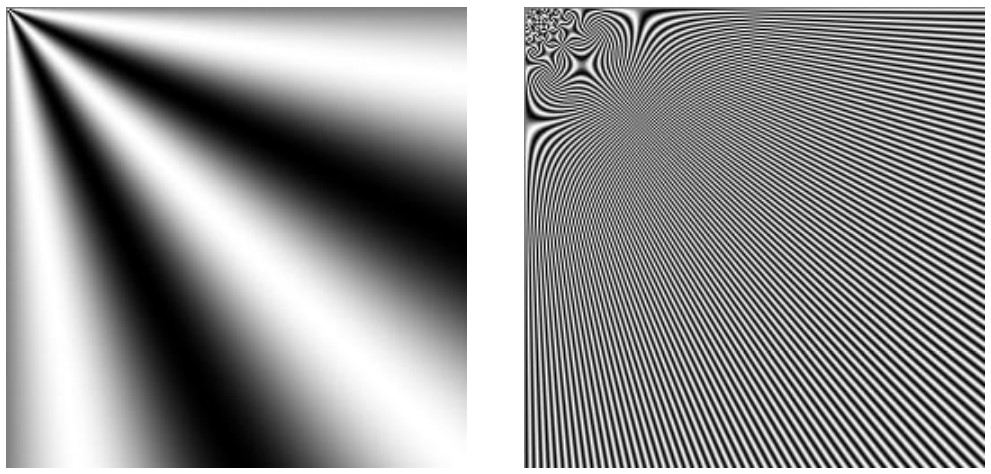
\includegraphics[width=10cm, keepaspectratio]{capitoli/immagini/imgs/aliasing_componenti_spettrali.jpg}
\end{figure}

L'aliasing deriva dal sottocampionamento e causa perdita di risoluzione
dell'immagine campionata (effetto scacchiera).

\begin{figure}[H]
    \centering
    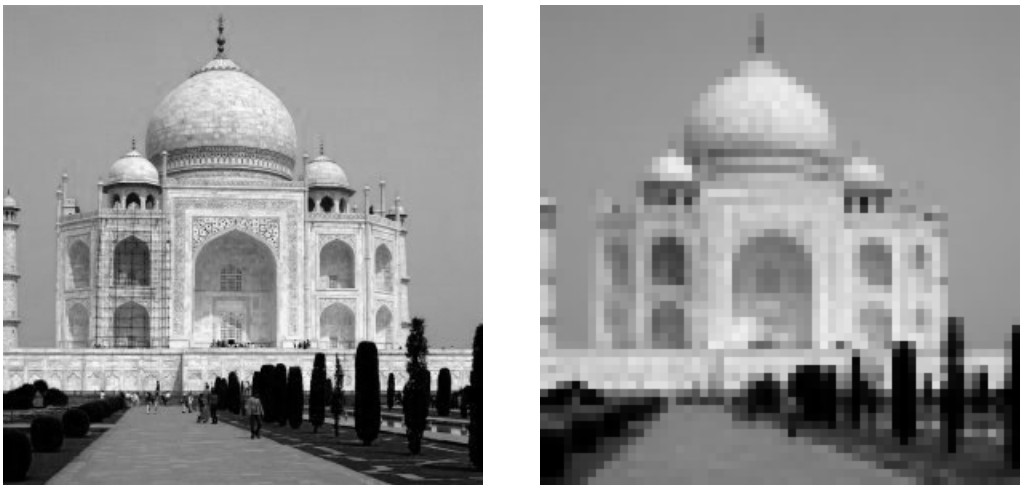
\includegraphics[width=10cm, keepaspectratio]{capitoli/immagini/imgs/aliasing_tajmahal.jpg}
\end{figure}

\paragraph{Note:} \TODO[]{Pricontrollare, potrebbe essere reso discorsivo.}
\begin{itemize}
    \item Per prevenire aliasing di queste componenti, è possibile filtrarle via
          (eliminarle) prima di campionare il segnale. Eliminare certe frequenze
          e lasciare passare le basse frequenze, è una operazione nota come
          \textbf{filtraggio passa-basso}.
    \item Ogni attenuazione relativa a questo processo di filtraggio rappresenta
          una perdita di risoluzione dell'immagine campionata.
    \item Come risultato, mentre da un lato c'è una perdita della risoluzione
          dell'immagine campionata, dall'altro c'è una attenuazione
          dell'aliasing error.
    \item \textbf{Effetto Moirè:} ovvero la distorsione visiva che si manifesta
          quando due griglie si sovrappongono
          \begin{figure}[H]
              \centering
              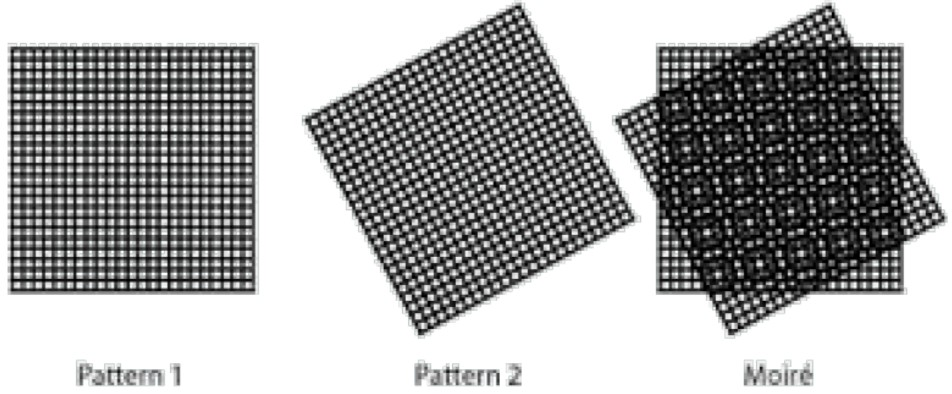
\includegraphics[width=8cm, keepaspectratio]{capitoli/immagini/imgs/effetto_moire.jpg}
          \end{figure}
\end{itemize}

\section{La risoluzione}
Il campionamento e la quantizzazione determinano la \textbf{risoluzione}
dell'immagine. \\\\La \textbf{risoluzione} di un segnale è un indice del grado
di qualità dell'immagine: misura il grado di oggetti distinguibili
nell'immagine. Esistono differenti definizione di risoluzione:

\begin{definition}
    La \textbf{Risoluzione Spaziale} indica la densità dei campioni, ovvero è data dal numero di campioni
    per unità di area.
\end{definition}

Spesso è espressa come numero di pixel
nell'unità di lunghezza e viene misurata in pixel per pollice (ppi).
\\Un'immagine ad alta risoluzione contiene più pixel di una delle
stesse dimensioni con una risoluzione inferiore, quindi è in grado di
riprodurre un maggior numero di dettagli. Un'elevata risoluzione
comporta tuttavia un aumento considerevole delle dimensioni (quantità
di dati) dell'immagine.

\paragraph{Esempio:}

Un'immagine di 1cm x 1cm con una risoluzione di 72 ppi
contiene 5184 pixel (72 x 72). La stessa immagine di 1 cm x
1 cm a 300 ppi conterrebbe 90.000 pixel.

\begin{definition}
    La \textbf{Risoluzione spettrale} indica la banda passante del sensore.

\end{definition}


\begin{definition}
    \textbf{Risoluzione radiometrica} indica il numero di livelli di quantizzazione.

\end{definition}


\begin{definition}
    \textbf{Risoluzione temporale} indica la frequenza di acquisizione dei frames di un'immagine in
    movimento.
\end{definition}



\section{Alterazioni della risoluzione}
Alterando i vari tipi di risoluzione, l'immagine presenterà di volta in volta un
diverso tipo di distorsione. \\ \textbf{Immagine originale:}

\begin{figure}[H]
    \centering
    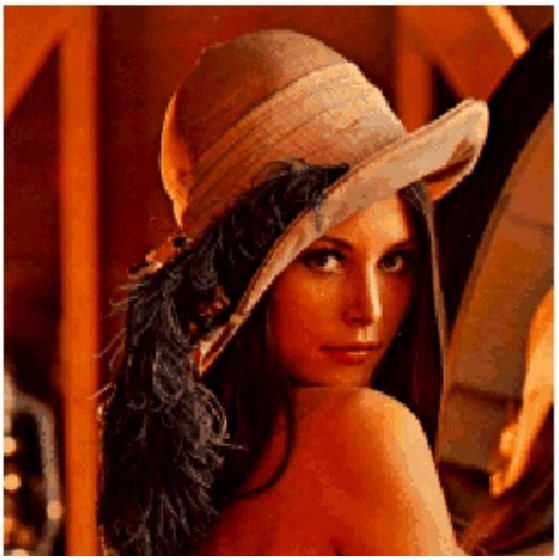
\includegraphics[width=4cm, keepaspectratio]{capitoli/immagini/imgs/alterazione_risoluzioni_esempio_base.jpg}
\end{figure}

\begin{trivlist}
    \item \textbf{Risoluzione spaziale:} diminuendo la risoluzione spaziale
    (nell'esempio di un quarto) si ottiene il tipico effetto ”quadrettato”,
    detto anche a scacchiera, dovuto all'aliasing.
    \begin{figure}[H]
        \centering
        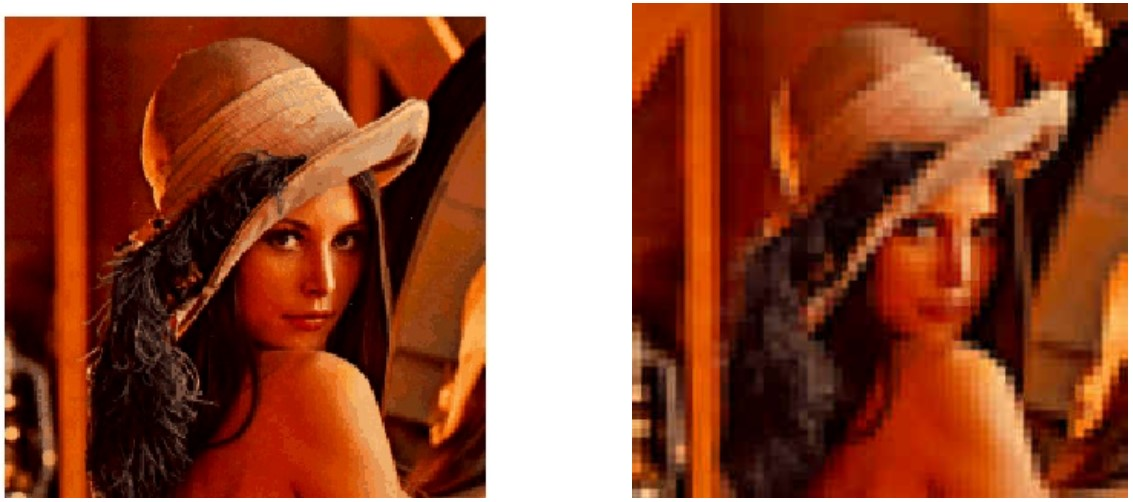
\includegraphics[width=10cm, keepaspectratio]{capitoli/immagini/imgs/esempio_risoluzione_spaziale.jpg}
    \end{figure}

    \item \textbf{Risoluzione spettrale:} Diminuendo la banda passante del
    sensore di acquisizione dell'immagine si ottiene un'immagine più ”sfocata”,
    in quanto i dettagli ad alta frequenza spaziale vanno persi.
    \begin{figure}[H]
        \centering
        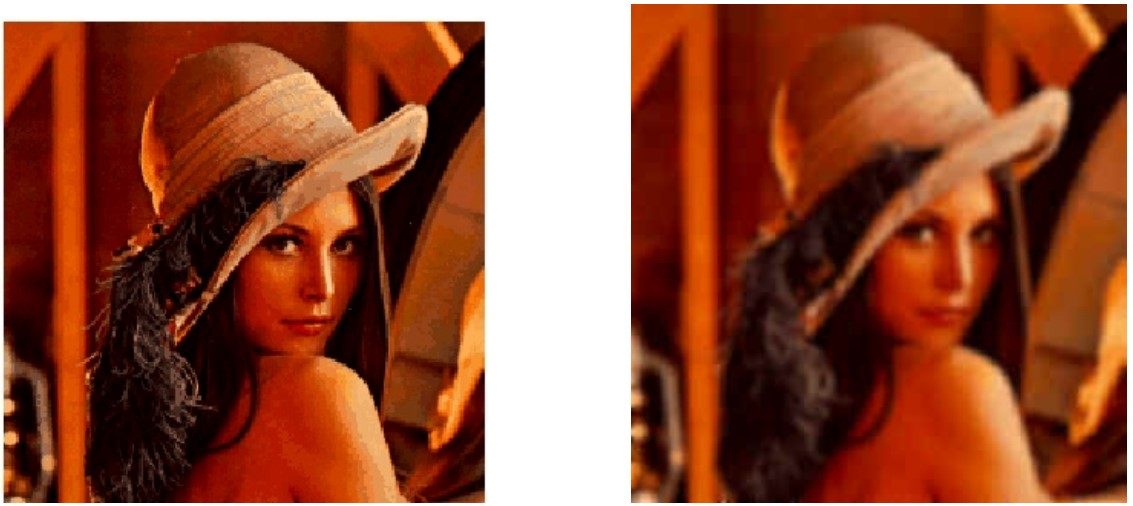
\includegraphics[width=10cm, keepaspectratio]{capitoli/immagini/imgs/esempio_risoluzione_spettrale.jpg}
    \end{figure}

    \item \textbf{Risoluzione radiometrica:} Diminuendo la profondità di colore,
    si distinguono in maniera più marcata i passaggi da un colore ad un altro;
    essi risultano pertanto sempre più accentuati e meno graduali, fino a
    produrre dei ”falsi contorni”
    \begin{figure}[H]
        \centering
        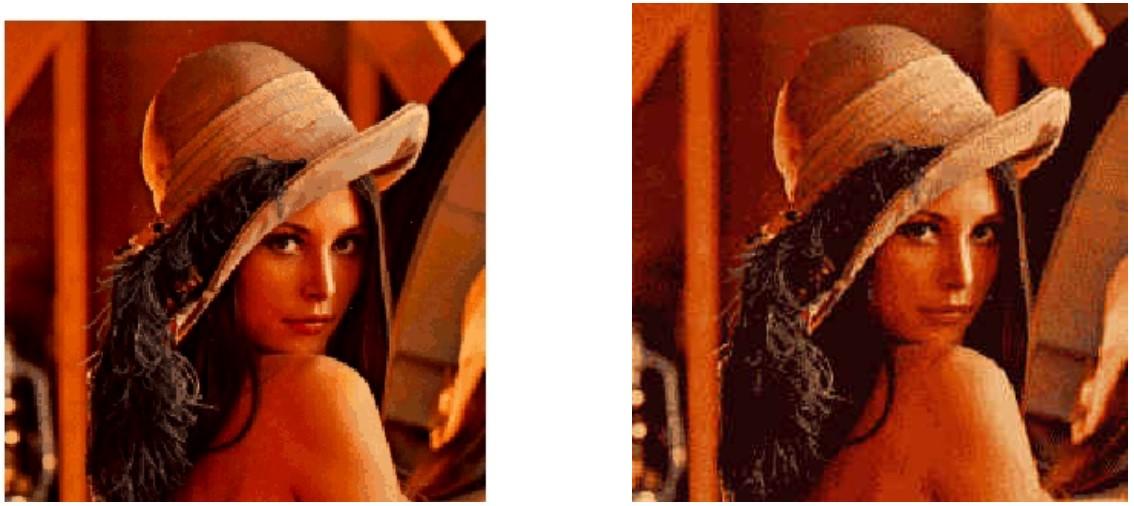
\includegraphics[width=10cm, keepaspectratio]{capitoli/immagini/imgs/esempio_risoluzione_radiometrica.jpg}
    \end{figure}
\end{trivlist}

\section{Immagini in bianco e nero e immagini a colori}

\subsection{Immagini in bianco e nero}

Un'\textbf{immagine in bianco e nero (b/w)} è caratterizzata da una
rappresentazione binaria, ovvero la funzione che la rappresenta in
ogni punto ($x$ , $y$) può assumere solo due valori: 0 e 1. In genere,
ad 1 si associa il bianco, mentre a 0 il nero.

\begin{figure}[H]
    \centering
    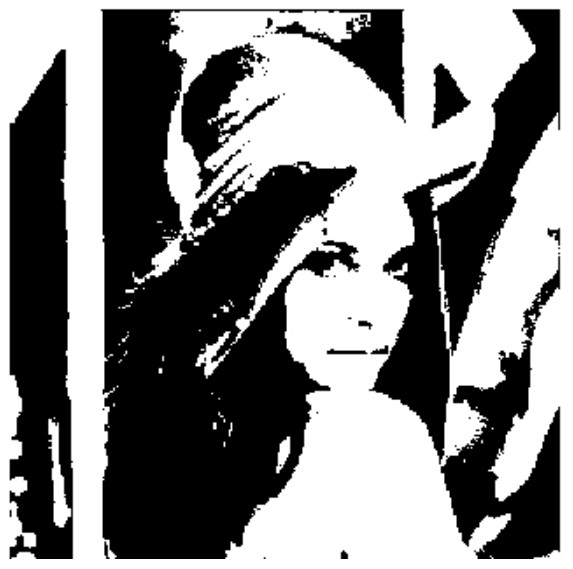
\includegraphics[width=4cm, keepaspectratio]{capitoli/immagini/imgs/immagine_binaria_bianco_nero.jpg}
\end{figure}

\subsection{Immagini a colori}

Per rappresentare un'\textbf{immagine a colori} è necessario ricorrere ad
una funzione vettoriale. Un colore infatti può essere sempre
decomposto come \textbf{somma dei tre colori fondamentali (rosso, verde,
    blu)}, ciascuno con un'opportuna intensità.
Un'immagine a colori, dunque, può essere rappresentata da una
funzione $f: \mathbb{R}^2 \rightarrow \mathbb{R}^3$ del tipo

$$
    f(x, y) = [R(x, y), G(x, y), B(x, y)]
$$

Questo tipo di rappresentazione viene detta \textbf{RGB (Red,Green,Blue)}.
\subsection{Lo spazio RGB}

Lo spazio RGB è uno spazio cartesiano, con tre assi ortogonali.
Il colore di ciascun pixel viene rappresentato da un vettore
$[R(x , y), G(x , y), B(x , y)]$ nello spazio RGB; ogni componente
indica la quantit`a di rosso, verde e blu, rispettivamente, necessari
ad ottenere quel colore.
In base alla rappresentazione RGB, un'immagine a colori viene
rappresentata da una terna di matrici, ognuna delle quali contiene i
valori relativi ad un canale di colore.\\
Ogni canale, preso a sè, non è altro che un'immagine a toni di
grigio.

\begin{figure}[H]
    \centering
    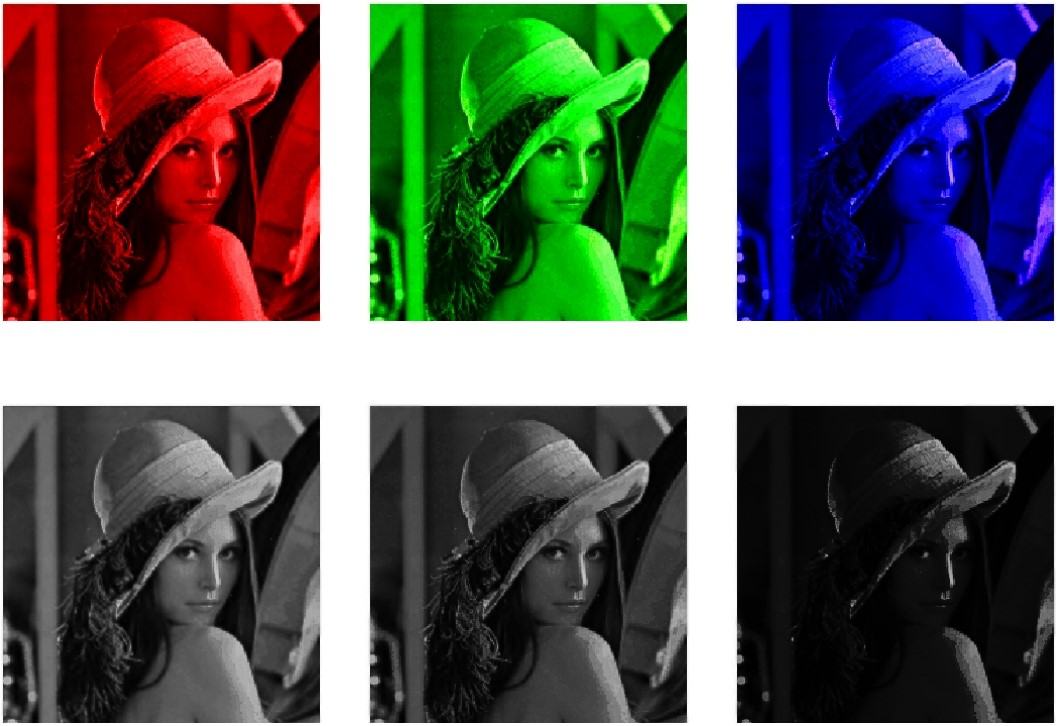
\includegraphics[width=12cm, keepaspectratio]{capitoli/immagini/imgs/canali_RGB_e_grigio.jpg}
\end{figure}

\subsection{Lo spazio HSV}

Oltre alla RGB esistono anche altri tipi di rappresentazioni (che
possono essere in genere derivate da essa).
Una di queste è la rappresentazione \textbf{HSV}. Lo spazio HSV ha un
sistema di coordinate cilindrico con due assi ortogonali ed un
angolo di rotazione intorno ad uno dei due assi.
L'altezza del cono rappresenta la \textbf{luminosità (Value)}, con valori da
0 (nero) a 1 (bianco). La \textbf{saturazione (Saturation)} indica l'intensità
e la purezza del colore, con valori da 0 (sull'asse del cono) a 1
(sulla superficie del cono). La terza coordinata rappresenta la
\textbf{tonalità di colore (Hue)} e viene misurata da un angolo intorno
all'asse verticale (rosso a 0 gradi, verde a 120 e blu a 240).

\begin{figure}[H]
    \centering
    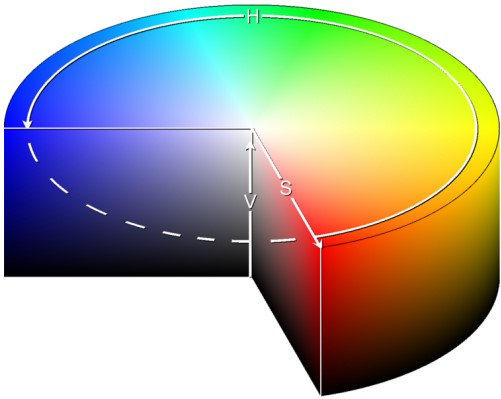
\includegraphics[width=5cm, keepaspectratio]{capitoli/immagini/imgs/cilindro_hsv.jpg}
\end{figure}

\section{Immagini a toni di grigio}

Un'immagine a toni di grigio è rappresentata da una matrice le cui
entrate sono i valori che la funzione $f$ assume in ogni punto.

\begin{figure}[H]
    \centering
    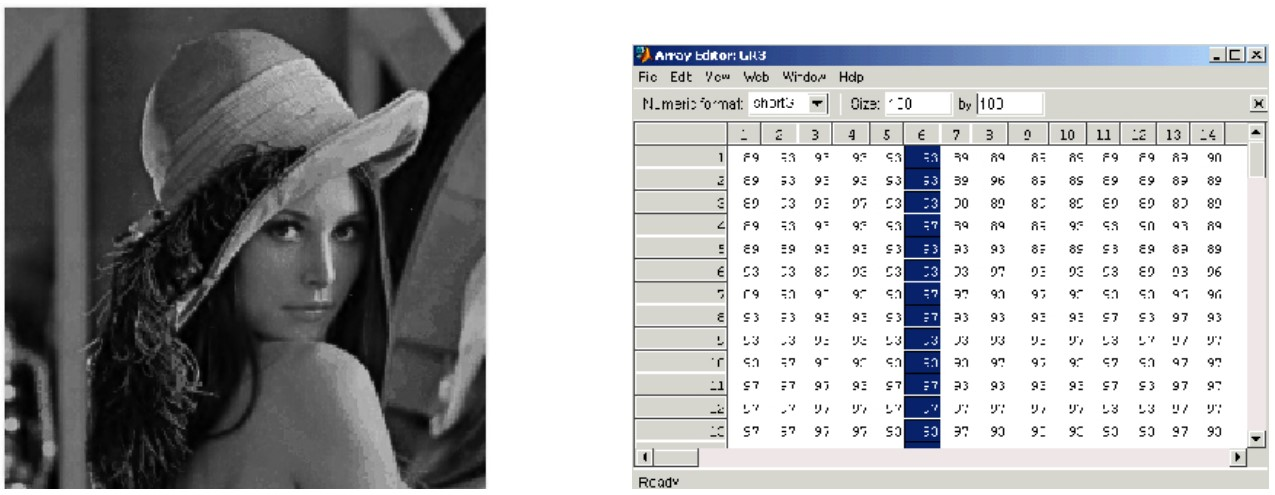
\includegraphics[width=12cm, keepaspectratio]{capitoli/immagini/imgs/rappresentazione_immagine_toni_grigio.jpg}
\end{figure}

In genere, si assume che i \textbf{livelli di grigio} siano discreti ed
equispaziati in un intervallo di valori normalmente \textbf{tra 0 e 255}:
esistono allora un massimo di 256 livelli di grigio.
\\
La funzione $f (x , y)$ può essere rappresentata come una superficie
nello spazio.

\begin{figure}[H]
    \centering
    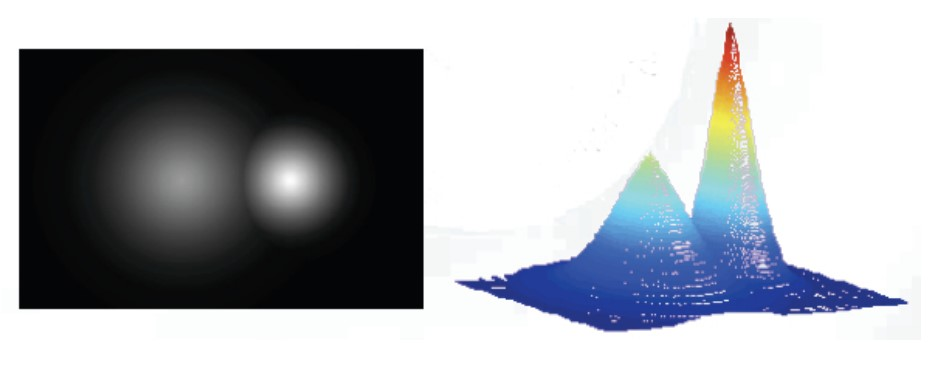
\includegraphics[width=10cm, keepaspectratio]{capitoli/immagini/imgs/funzione_toni_grigio.jpg}
\end{figure}

\subsection{Zoom e Shrink}

\TODO[inline]{DA IMPLEMENTARE QUANDO IL PROF LE SPIEGA}

\subsection{Elaborazione delle immagini}
L'elaborazione delle immagini è una disciplina che prevede l'utilizzo
di algoritmi i quali operano sui pixel che compongono l'immagine
e, applicando trasformazioni numeriche, restituiscono un'immagine
modificata.\\
Le tecniche di elaborazione delle immagini hanno vari scopi, fra cui:

\begin{itemize}
    \item il miglioramento della qualità dell'immagine (\textbf{image enhancement})
    \item il ripristino della qualità dell'immagine (\textbf{image restoration})
    \item l'estrazione di informazioni sul contenuto dell'immagine (\textbf{image analysis})
\end{itemize}

\paragraph{Note:}

\begin{itemize}
    \item L'\textbf{image analysis} è una parte fondamentale della computer vision e
          precede l'\textbf{image recognition}.\\
          Essa può richiedere elaborazioni differenti a seconda del tipo di
          informazione che si vuole estrarre: tra queste, le elaborazioni nel
          dominio spaziale, nel dominio delle frequenze, con riduzione dei
          dati tra ingresso e uscita (compressione), etc.
\end{itemize}

\paragraph{Esempio:}

Un'elaborazione nel dominio spaziale, ad esempio, può essere
espressa come

$$
    g(x , y) = T(f (x , y))
$$

\begin{itemize}
    \item $f$ è l'immagine di ingresso
    \item $g$ è l'immagine di uscita
    \item $T$ è un operatore su f, definito in un intorno di $(x , y)$.
\end{itemize}

La natura dell'intorno definisce il tipo di elaborazione e si distingue,
in particolare, fra: \textbf{elaborazioni puntuali}, \textbf{locali} e \textbf{globali}.

\begin{definition}
    Le elaborazioni \textbf{puntuali} trasformano il valore di un pixel sulla base del
    valore del pixel stesso.
\end{definition}

\begin{definition}
    Le elaborazioni \textbf{locali} lavorano sulla base dei valori assunti dai pixel in
    un intorno di quello preso in esame.
\end{definition}

\begin{definition}
    Le elaborazioni \textbf{globali} trasformano il valore di un pixel sulla
    base dei valori assunti da tutti i pixel dell'immagine.
\end{definition}

\subsubsection{Elaborazioni Puntuali}

\begin{definition}
    Un'elaborazione puntuale si dice \textbf{omogenea} se il risultato
    dipende solo dal valore del pixel a cui è applicata.\\
    Se invece il risultato dipende anche dalla posizione del pixel,
    l'elaborazione puntuale è \textbf{non omogenea}.
\end{definition}

\paragraph{Note:}

\begin{itemize}
    \item Elaborazioni puntuali sono anche dette \textbf{manipolazioni della scala dei
              grigi}\\
          Un'elaborazione puntuale omogenea può essere rappresentata da
          una trasformazione

          $$
              s = T(r)
          $$

          \begin{itemize}
              \item $r$ è il livello di grigio dell'immagine di ingresso
              \item $s$ è il livello di grigio dell'immagine in uscita
          \end{itemize}
    \item In base al tipo di funzione T si ottiene un tipo diverso di
          trasformazione: a \textbf{gradino (threshold)}, a \textbf{rampa},
          \textbf{lineare} a \textbf{tratti}...

          \begin{figure}[H]
              \centering
              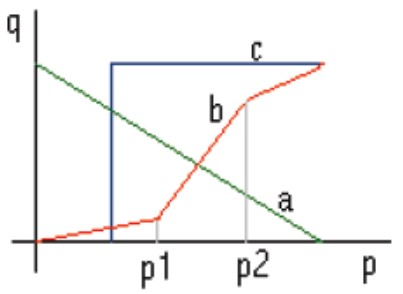
\includegraphics[width=5cm, keepaspectratio]{capitoli/immagini/imgs/elaborazioni_puntuali_immagine.jpg}
          \end{figure}

\end{itemize}

\paragraph{Esempio 1.} \ \\

Consideriamo una funzione T a gradino, ottenendo così una
\textbf{elaborazione threshold (soglia)}.\\
Tale elaborazione fa sì che i valori dei pixel che non superano la
soglia fissata vengano portato a 0, mentre i valori dei pixel che
superano la soglia siano posti pari a 1.\\
Si produce così un'immagine \textbf{binaria}.

\begin{figure}[H]
    \centering
    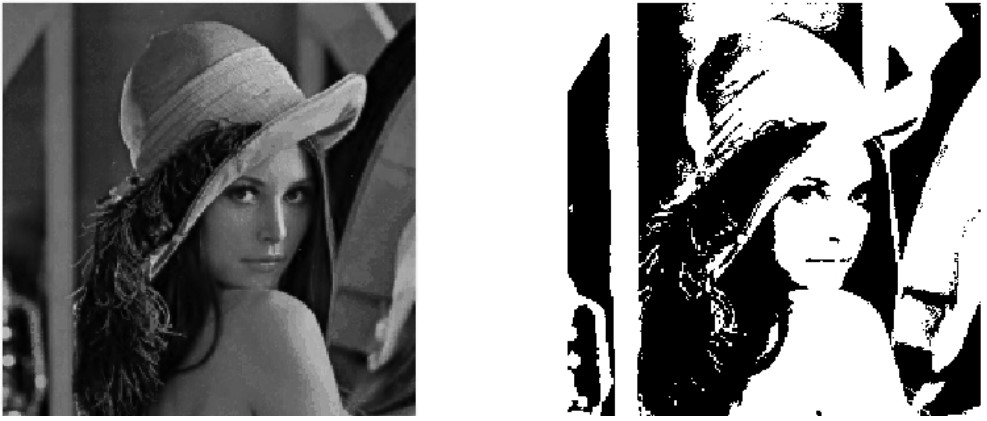
\includegraphics[width=10cm, keepaspectratio]{capitoli/immagini/imgs/foto_esempio_1.jpg}
\end{figure}

Questo è un tipico esempio di \textbf{binarizzazione}.
Si può ottenere una binarizzazione anche scegliendo una qualsiasi
altra \textbf{funzione di discriminazione}, invece di una soglia costante.

\paragraph{Esempio 2.}\ \\

Consideriamo una $T$ del tipo:

\begin{figure}[H]
    \centering
    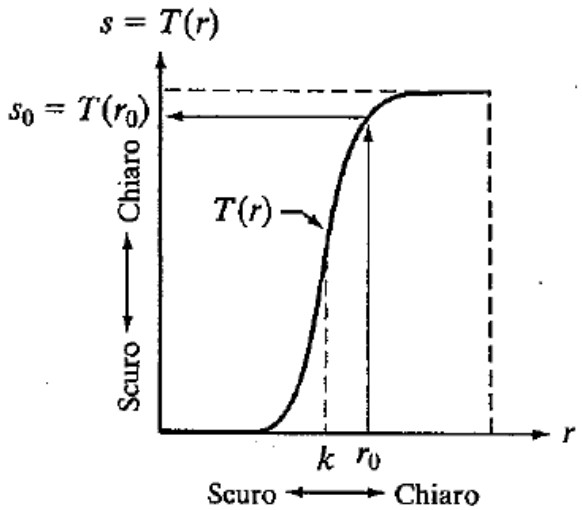
\includegraphics[width=6cm, keepaspectratio]{capitoli/immagini/imgs/trasformazione_esempio_2.jpg}
\end{figure}

Vengono scuriti i livelli di grigio al di sotto di $k$ e schiariti quelli al
di sopra di $k$. Si ottiene così uno \textbf{stiramento dell'immagine (image
    stretching)}. L'elaborazione threshold può essere riguardata come
caso limite di questo tipo di operazione.

\paragraph{Esempio 3.}\ \\

Consideriamo una $T$ del tipo:

$$
    T(r) = L - 1 - r
$$

se il range dinamico dell'immagine è $[0, L - 1]$
la scala di grigi viene invertita, ottenendo così una negazione.

\begin{figure}[H]
    \centering
    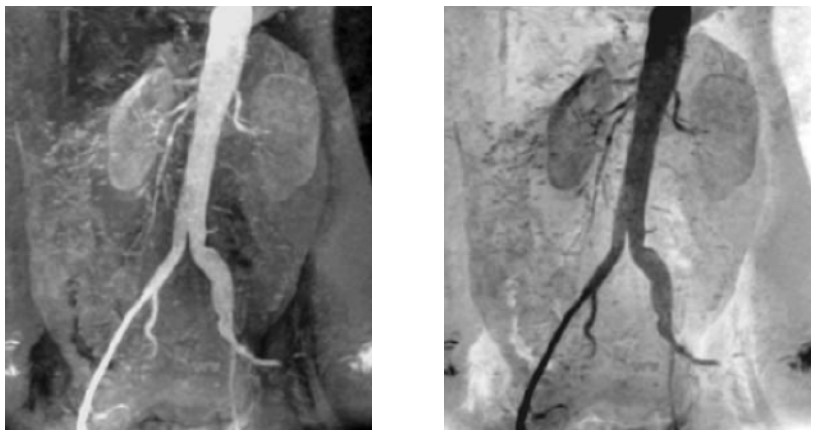
\includegraphics[width=8cm, keepaspectratio]{capitoli/immagini/imgs/angiografie_esempio_3.jpg}
\end{figure}

\paragraph{Esempio 4.}\ \\

Consideriamo una $T$ del tipo:

$$
    T(r) = c \log(1 + r), c \in  \mathbb{R}, r \geq 0
$$

che prende il nome di \textbf{trasformazione logaritmica}: associa ad una
stretta gamma di valori a bassa intensità dell'immagine originale
una più ampia gamma nell'immagine in output.\\
Per livelli ad alta intensità, invece, si verifica il contrario.\\
Un tipico caso in cui è utile applicare questa trasformazione è per
rappresentare la trasformata di Fourier, che spesso presenta una
gamma molto ampia di intensità, difficilmente riproducibile senza
perdere un significativo livello di dettaglio

\begin{figure}[H]
    \centering
    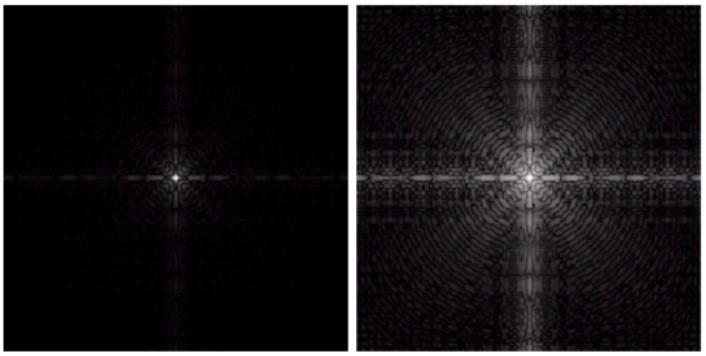
\includegraphics[width=10cm, keepaspectratio]{capitoli/immagini/imgs/trasformazione_logaritmica_esempio_4.jpg}
\end{figure}

\begin{itemize}
    \item Fig. sinistra: spettro di Fourier con valori in $[0, 1.5 \times 10^6]$.
    \item Fig. destra: risultato dell'applicazione della trasformazione logaritmica
          con $c = 1$ (valori in $[0, 6.2]$).
\end{itemize}

\paragraph{Esempio 5.}\ \\

Consideriamo una $T$ del tipo:

$$
    T(r) = cr^\gamma, c, \gamma > 0,
$$

che prende il nome di \textbf{trasformazione di potenza (gamma)}
Se $\gamma < 1$ le curve potenza corrispondenti trasformano una stretta
gamma di valori scuri in una gamma più ampia di valori in output,
mentre se $\gamma > 1$, si verifica la trasformazione opposta.\\
La correzione tramite il fattore $\gamma$ è importante per la corretta
visualizzazione di immagini sullo schermo di un computer:
immagini non corrette nel modo giusto possono apparire sbiadite o,
al contrario, troppo scure.

\begin{figure}[H]
    \centering
    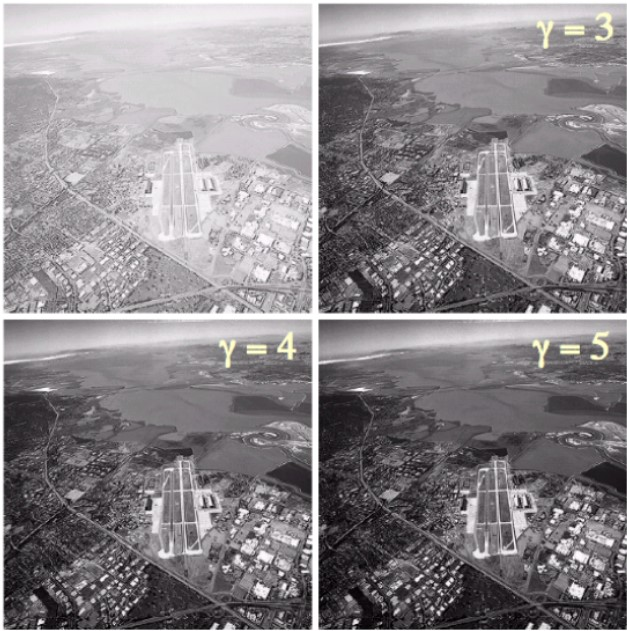
\includegraphics[width=6cm, keepaspectratio]{capitoli/immagini/imgs/foto_esempio_5.jpg}
\end{figure}

\paragraph{Esempio 6.}\ \\

Considerando una $T$ \textbf{lineare a tratti} del tipo si ottiene uno
stretching del contrasto

\begin{figure}[H]
    \centering
    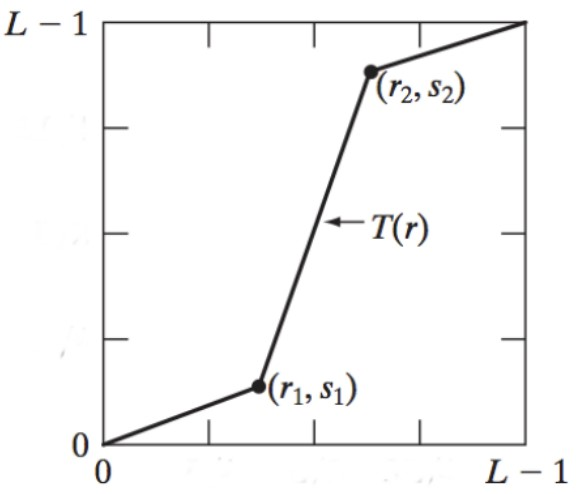
\includegraphics[width=5cm, keepaspectratio]{capitoli/immagini/imgs/lineare_a_tratti_esempio_6.jpg}
\end{figure}

In questo caso invece si ha uno stretching del contrasto differente perché si
sceglie come $(r_1, s_1) = (r_{min}, 0)$ e $(r_2, s_2) = (r_{max} , L - 1)$

\begin{figure}[H]
    \centering
    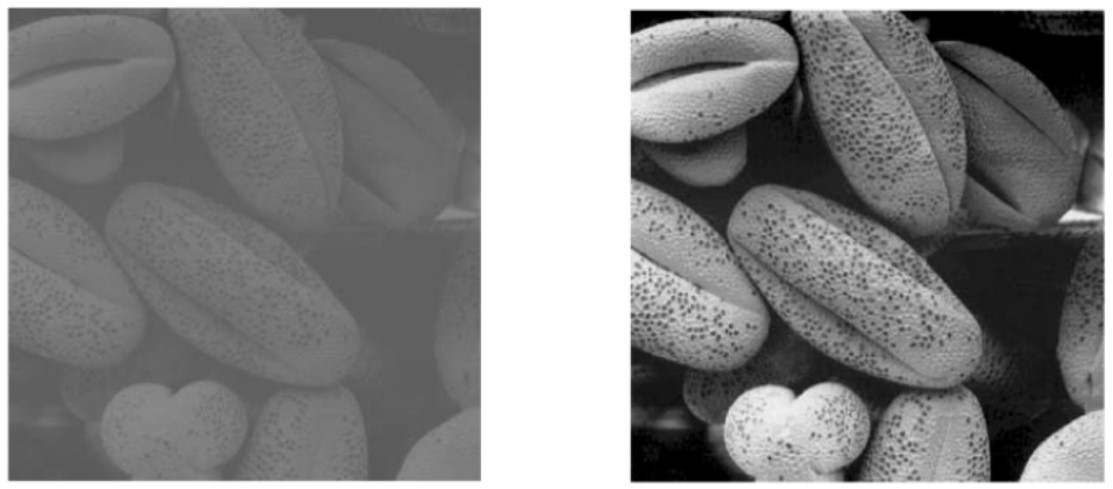
\includegraphics[width=10cm, keepaspectratio]{capitoli/immagini/imgs/globuli_rossi.jpg}
\end{figure}

\paragraph{Note:}
\begin{itemize}
    \item In questo caso $r_{min}$ e $r_{max}$ stanno ad indicare il più basso e alto valore
          nei livelli di grigio dell'immagine utilizzata.
\end{itemize}

\paragraph{Esempio 7.}\ \\

\begin{figure}[H]
    \centering
    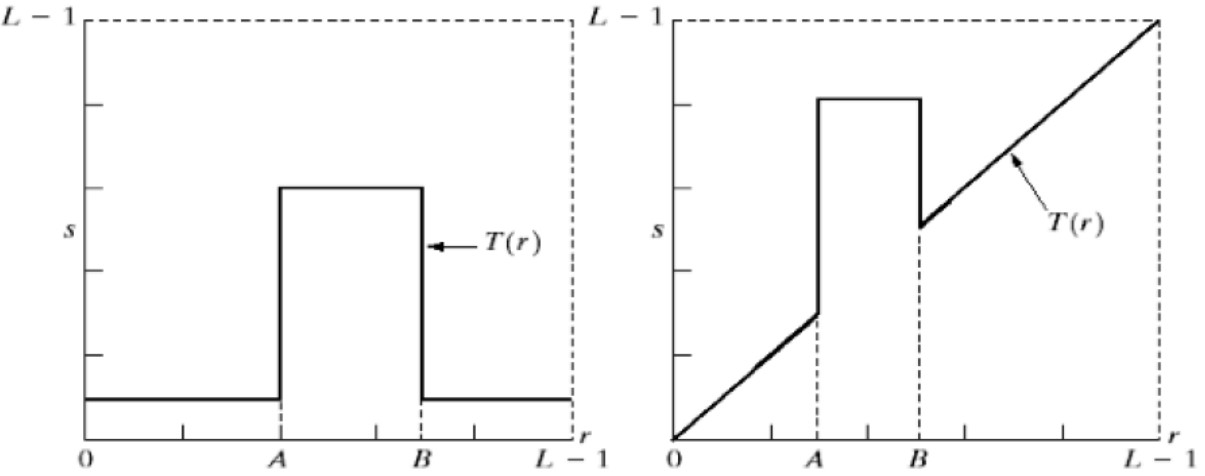
\includegraphics[width=\linewidth, keepaspectratio]{capitoli/immagini/imgs/trasformazioni_lineari_esempio_7.jpg}
\end{figure}

In questo caso prendiamo queste due diverse trasformazioni ed analizziamo il loro effetto sull'immagine.

\begin{itemize}
    \item La prima crea una binarizzazione ma in questo caso utilizza due differenti gradazioni di grigio e sono precisamente bianco e nero.
    \item La seconda mette in \textbf{risalto} una porzione della scala di grigi alzandogli il livello e schiarendoli.
\end{itemize}

\begin{figure}[H]
    \centering
    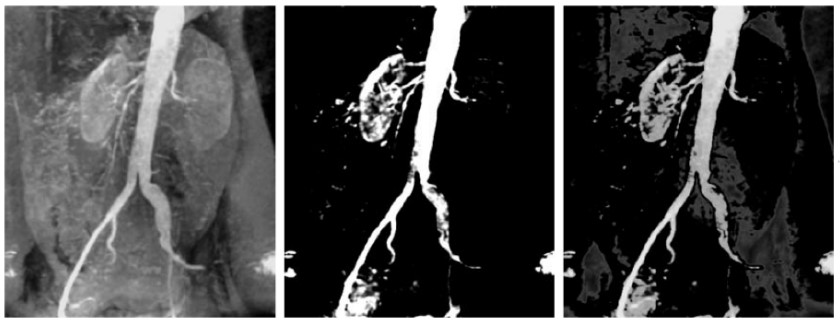
\includegraphics[width=\linewidth, keepaspectratio]{capitoli/immagini/imgs/angiografie_esempio_7.jpg}
\end{figure}

\begin{itemize}
    \item Nella prima immagine vediamo una normale Angiografia aortica.
    \item Nella seconda abbiamo il risultato della selezione di intensità del primo tipo (banda di
          interesse $[A, B]$ selezionata sulla parte alta della scala di grigi).
    \item Nella terza abbiamo il risultato della selezione di intensità del secondo tipo (banda
          $[A, B]$ sulle tonalità medio-grigie impostata sul nero, così da
          preservare le tonalità di grigio dei vasi e dei reni).
\end{itemize}

\subsubsection{Finestramento - Windowing}

\begin{definition}
    \textbf{Il windowing} consiste nel mostrare solo una parte del range dei valori di grigio dell’immagine.
\end{definition}

\begin{figure}[H]
    \centering
    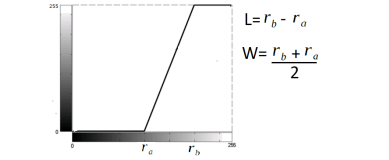
\includegraphics[width=\linewidth, keepaspectratio]{capitoli/immagini/imgs/win1.png}
\end{figure}

\textbf{Applicazione:} in molte immagini mediche il numero di valori della
scala dei grigi utili dal punto di vista diagnostico `e sensibilmente
minore di tutti quelli disponibili. Usando sul monitor tutto il range
possibile si diminuisce il contrasto visibile nella zona di interesse.

\begin{figure}[H]
    \centering
    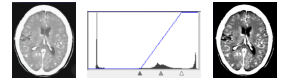
\includegraphics[width=\linewidth, keepaspectratio]{capitoli/immagini/imgs/windowing.png}
\end{figure}

\begin{itemize}
    \item Finestramento con $L = 169$ e $W = 97$
    \item Numero di grigio: $238$ (Immagine di sx) e $97$ (immagine di dx)
    \item Non viene aggiunta informazione, si aumenta solo il contrasto visibile
\end{itemize}

\section{Modelli delle Immagini}
In base al tipo di elaborazione che si vuole effettuare, può essere conveniente adottare diversi modelli per le immagini. Ad esempio:

\begin{itemize}
    \item \textbf{Modello Deterministico}
    \item \textbf{Modello Probabilistico} (sui \textbf{pixel} prevedendo il che il valore dei pixel sia considerato una variabile aleatoria,
          oppure \textbf{sull'immagine} riguardando cioè l'immagine stessa come un processo stocastico)
\end{itemize}

\subsection{Il modello Probabilistico}

Nel modello probabilistico per i pixel, i valori assunti nei vari pixel ($N × M$) di un’immagine vengono considerati come valori assunti
da una variabile aleatoria in una successione di $N × M$ esperimenti. E’ dunque possibile analizzare ed elaborare l’immagine utilizzando gli strumenti del calcolo delle probabilità e del calcolo stocastico.
Un esempio di questo processo è \textbf{l’analisi dell’istogramma}.

\section{L’istogramma dei toni di grigio}

\textbf{L’istogramma dei toni di grigio} (istogramma) si ottiene contando, per ogni valore del codominio dell’immagine (spazio di tutti i valori
che possono essere assunti dai pixel), il numero di volte che tale valore compare nell’immagine.
Il grafico che si ricava è un istogramma, cioè un grafico a barre dove l’asse delle ascisse è suddiviso in tanti punti quanti sono i
possibili toni di grigio dell’immagine.

\begin{trivlist}
    \item \textbf{Esempio}: il codominio di un’immagine a 256 toni di grigio sarà formato da tutti i numeri interi da 0 a 255 $\rightarrow$ l’asse orizzontale sarà suddiviso in 256 parti.
\end{trivlist}

\begin{figure}[H]
    \centering
    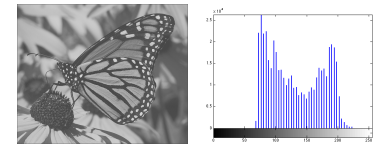
\includegraphics[width=\linewidth, keepaspectratio]{capitoli/immagini/imgs/esempio-istogramma.png}
\end{figure}

\textbf{In termini probabilistici:} l’istogramma rappresenta la distribuzione di probabilità della variabile aleatoria r che indica il
valore di grigio di un pixel.

\begin{definition}
    In base alla definizione di distribuzione l’istogramma andrebbe normalizzato in modo da assumere valori tra 0 e 1.
    Se i toni di grigio sono $r_k, k = 0, . . . , 255$ allora l’altezza della barra in $r_k$ è pari alla frequenza relativa di $r_k$ , ovvero
    \begin{center}
        $p(r_k) = \frac{n_k}{n}$
    \end{center}
    dove $n_k$ è il numero di pixel in cui viene assunto $r_k$, $n$ è il numero totale di pixel dell'immagine.
\end{definition}

L’istogramma quindi fornisce una raffigurazione sintetica del contenuto cromatico o di luminosità dell’immagine, dunque una descrizione
della qualità dell’immagine.

\begin{itemize}
    \item \textbf{Esempio:} \textbf{Immagine troppo scura}
          la distribuzione è concentrata su toni bassi di grigio
\end{itemize}

\begin{figure}[H]
    \centering
    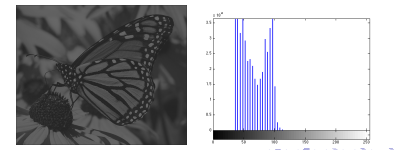
\includegraphics[width=\linewidth, keepaspectratio]{capitoli/immagini/imgs/isto-scuro.png}
\end{figure}

\begin{itemize}
    \item \textbf{Esempio:} \textbf{Immagine troppo chiara}
          la distribuzione è concentrata su toni alti di grigio
\end{itemize}

\begin{figure}[H]
    \centering
    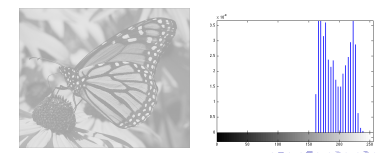
\includegraphics[width=\linewidth, keepaspectratio]{capitoli/immagini/imgs/isto-chiaro.png}
\end{figure}

\begin{itemize}
    \item \textbf{Esempio:} \textbf{Immagine con alto contrasto}
          la distribuzione è concentrata su valori vicini a 0 e a 255
\end{itemize}

\begin{figure}[H]
    \centering
    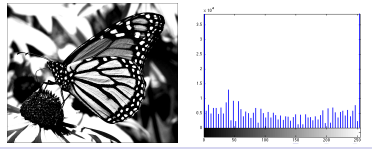
\includegraphics[width=\linewidth, keepaspectratio]{capitoli/immagini/imgs/alto-c.png}
\end{figure}

\subsection{Interventi sull’istogramma}
Qualora le caratteristiche della distribuzione dei toni di grigio nell’immagine non siano ottimali, è consigliabile applicare
all’istogramma opportune trasformazioni, basate su sistemi stocastici.
Tra queste:

\begin{itemize}
    \item \textbf{Equalizzazione dell’istogramma}
    \item \textbf{Shift dell’istogramma}
    \item \textbf{Stretching dell’istogramma}
\end{itemize}

\subsubsection{Equalizzazione sull'istogramma}

\textbf{L'equalizzazione dell’istogramma} ha lo scopo di uniformare l’istogramma dell’immagine lungo tutto il suo dominio. Il risultato
è un nuovo istogramma in cui il numero di pixel ad ogni tono di grigio è il più possibile costante.
\\\textbf{Algoritmo:}

\begin{center}
    $T(r_k) = (L-1)\sum_{j=0}^{k}p(r_j)=\frac{L-1}{n} \sum_{j=0}^{k}n_j = \frac{L-1}{MN}\sum_{j=0}^{k}n_j$
\end{center}

$k=0,...,L-1$.
\\\textbf{Il risultato} è l'aumento del contrasto.

\subsubsection{Risultato equalizzazione dell'istogramma}

\begin{figure}[H]
    \centering
    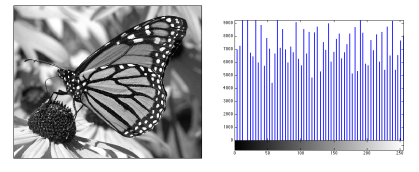
\includegraphics[width=\linewidth, keepaspectratio]{capitoli/immagini/imgs/eq-istogramma.png}
\end{figure}

\subsubsection{Equalizzazione sull'istogramma}

\textbf{Shift dell’istogramma:} consiste nel traslare i valori dell’istogramma.
\\\textbf{Algoritmo:}
\begin{center}
    $T(r) = \alpha r, 0 < \alpha < 1$
    \\
    $T(r) = \alpha r + (L-1)(1-\alpha), 0<\alpha<1$
\end{center}
Il $risultato$ è un immagine più scura o schiarita.

\subsubsection{Risultato shift dell'istogramma}

\begin{figure}[H]
    \centering
    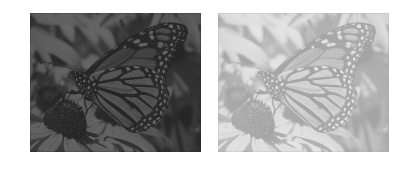
\includegraphics[width=\linewidth, keepaspectratio]{capitoli/immagini/imgs/shift-isto.png}
\end{figure}

\subsubsection{Stretching dell’istogramma}

si usa quando l’istogramma presenta dei picchi abbastanza ravvicinati, provocando un’immagine
piuttosto uniforme. Consiste in uno $stiramento$ dell’istogramma, in modo da distanziarne i picchi.
\\\textbf{Algoritmo:}
\begin{center}
    $$
        T(r) = \left\{ \begin{array}{cl}
            0                                         & \ 0 <= r <= r_{min}       \\
            (r - r_{min}) \frac{L-1}{r_{max}-r_{min}} & \ r_{min} <= r <= r_{max} \\
            L-1                                       & \ r_{max} <= r <= L-1
        \end{array} \right.
    $$
\end{center}
dove $[r_min, r_max ]$ è il range osservato nell’immagine originale, individuato dal minimo e dal massimo livello di grigio che presenta
l’immagine.
\\Il risultato è \textbf{l'aumento di contrasto}

\subsubsection{Risultato strtching dell'istogramma}

\begin{figure}[H]
    \centering
    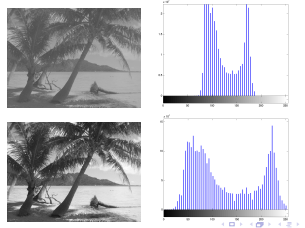
\includegraphics[width=\linewidth, keepaspectratio]{capitoli/immagini/imgs/stretch-isto.png}
\end{figure}

\section{Il rumore}

Per \textbf{rumore} si intende l’insieme dei segnali indesiderati che si sovrappongono al segnale utile oggetto di studio (ad esempio un’immagine) causandone una degenerazione.
\\
Si possono avere diverse forme di degrado tra cui, ad esempio:
\begin{itemize}
    \item \textbf{Il rumore di quantizzazione}
    \item \textbf{Il rumore introdotto da condizioni esterne}
    \item \textbf{Il rumore introdotto dal sensore}
    \item \textbf{Il rumore introdotto dai dispositivi di amplificazione/condizionamento del segnale}
\end{itemize}

In base alle sue cause, il rumore si distingue tra:
\begin{itemize}
    \item \textbf{Rumore indipendente dal segnale} (additivo)
    \item \textbf{Rumore dipendente dal segnale} (la relazione tra il segnale corrotto e quello originale è non lineare)
\end{itemize}

\begin{trivlist}
    \item \textbf{Rumore indipendete dal segnale:} (caso più comune) la funzione che descrive il segnale corrotto è:
    \begin{center}
        $f(x,y) = g(x,y)+v(x,y)$
    \end{center}
    dove $g(x,y)$ è il segnale e $v(x,y)$ è il rumore $\rightarrow$ \textbf{additivo}
    \item \textbf{Rumore dipendente dal segnale:} l’intensità del rumore dipende dal
    segnale. Supponendo anche che esso sia molto più grande del segnale, la funzione è
    \begin{center}
        $f(x,y)=g(x,y)+v(x,y)g(x,y)=g(x,y)(1+v(x,y)) \approx g(x,y)v(x,y)$
    \end{center}
    $\rightarrow$ \textbf{moltiplicativo}
\end{trivlist}

Essendo di natura intrinsecamente stocastica, il rumore viene in
genere analizzato usando la teoria dei processi stocastici ed è
caratterizzato in base alla:

\begin{itemize}
    \item \textbf{Distribuzione:} descrive la probabilità che il rumore assuma
          certi valori di intensità
    \item \textbf{Distribuzione spettrale:} ha a che fare con l’energia ad esso
          associata, al variare della frequenza
\end{itemize}

\subsection{Il modello del rumore}

Per poter caratterizzare e studiare il rumore in un’immagine si fanno in genere delle ipotesi semplificative, in modo che il rumore abbia una qualche distribuzione di probabilità: si costruisce in
questo modo un modello del rumore.
Una modellizazione tipica prevede che:

\begin{itemize}
    \item \textbf{lo spettro abbia distribuzione uniforme (rumore bianco)}
    \item \textbf{il rumore abbia distribuzione gaussiana, cioè}
          \begin{center}
              $p(r)=\frac{1}{\sigma \sqrt{2 \pi}}e^{-\frac{(r-\mu)^2}{2\sigma^2}}$
          \end{center}
          dove $\mu$ è il valor medio e $\sigma$ la deviazione standard.
\end{itemize}

%Inserire foto funzione

\subsubsection{Esempio}

\begin{figure}[H]
    \centering
    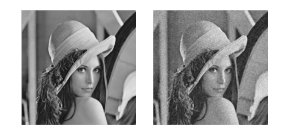
\includegraphics[width=\linewidth, keepaspectratio]{capitoli/immagini/imgs/esempio-rumore.png}
    \caption*{Immagine originale e immagine corrotta da rumore gaussiano}
\end{figure}

\subsubsection{Il rumore "salt and pepper"}

Nel caso in cui il rumore abbia distribuzione spaziale di tipo impulsivo, si parla di rumore salt and pepper (sale e pepe): agisce
corrompendo in maniera casuale i pixel dell’immagine, portandone il valore a $0=a$ (valore minimo) oppure a $255=b$ (valore massimo).
\begin{center}
    $$
        p(r) = \left\{ \begin{array}{cl}
            p_a & \ r = a    \\
            p_b & r = b      \\
            0   & altrimenti
        \end{array} \right.
    $$
\end{center}
Ovviamente il rumore impulsivo, pur essendo additivo, \textbf{non è
    lineare.}

%Inserire foto funzione

\subsubsection{Esempio}

\begin{figure}[H]
    \centering
    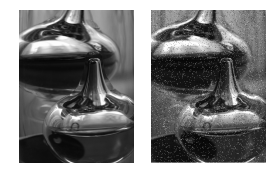
\includegraphics[width=\linewidth, keepaspectratio]{capitoli/immagini/imgs/esempio-salt-pepper.png}
    \caption*{Immagine originale e immagine corrotta da rumore salt and pepper}
\end{figure}

\subsubsection{Altre modellizzazioni del rumore: il rumore di Rayleigh}
\textbf{Il rumore di Rayleigh} ha la seguente distribuzione:

%Inserire foto funzione

\begin{center}
    $$
        p(r) = \left\{ \begin{array}{cl}
            \frac{2}{b}(r-a)e^{-{r-a}\frac{2}{b}} & \ r >= a \\
            0                                     & r<a
        \end{array} \right.
    $$
\end{center}

dove il valor medio e la deviazione standard sono dati da:

\begin{center}
    $\mu = a + \sqrt{\pi b/4}$ $\sigma = \frac{b(4-\pi)}{4}$
\end{center}

Nel grafico lo scostamento dall’origine e la forma inclinata verso
destra rende questa densit`a utile per l’approssimazione di
istogrammi non simmetrici e pu`o essere utilizzata per rappresentare
fenomeni di rumori tipici di alcuni sensori di range.

\subsubsection{Esempio}

\begin{figure}[H]
    \centering
    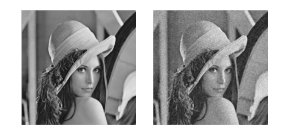
\includegraphics[width=\linewidth, keepaspectratio]{capitoli/immagini/imgs/esempio-rumore.png}
    \caption*{Immagine originale e immagine corrotta da rumore Rayleigh}
\end{figure}

\subsubsection{Altre modellizzazioni del rumore: il rumore Gamma}

Il \textbf{rumore gamma} ha la seguente distribuzione:

\begin{center}
    $$
        p(r) = \left\{ \begin{array}{cl}
            \frac{a^b r^{b-1}}{(b-1)!}e^-{ar} & \ r >= a \\
            0                                 & r<a
        \end{array} \right.
    $$
\end{center}

dove $a > 0$, $b$ è un intero positivo e il valor medio e la deviazione standard sono dati da:

\begin{center}
    $\mu=\frac{b}{a}$ $\sigma=\frac{\sqrt{b}}{a}$
\end{center}

Questo rumore è presente nelle immagini laser.

\subsubsection{Altre modellizzazioni del rumore: il rumore Esponenziale}

Il \textbf{rumore Esponenziale} ha la seguente distribuzione:

\begin{center}
    $$
        p(r) = \left\{ \begin{array}{cl}
            ae^{-ar} & \ r >= a \\
            0        & r<0
        \end{array} \right.
    $$
\end{center}
dove $a > 0$, b e il valor medio e la deviazione standard sono dati da:

%Inserire foto funzione

\begin{center}
    $\mu = \frac{1}{a}$ $\sigma = \frac{1}{a}$
\end{center}

Questo rumore è un caso particolare del rumore di Gamma con $b = 1$.

\subsubsection{Esempio}

\begin{figure}[H]
    \centering
    
\includegraphics[width=\linewidth, keepaspectratio]{capitoli/immagini/imgs/esempio-esponenziale.png}
    \caption*{Immagine originale e immagine corrotta da rumore Esponenziale}
\end{figure}

\subsubsection{Signal-Noise Ratio}

Per avere una valutazione numerica dell’entità del rumore associato ad una data immagine si pu`o ricorrere al \textbf{rapporto segnale-rumore
    (Signal Noise Ratio - SNR)}, definito come:

\begin{center}
    $
        SNR = \frac{\sum_{(x,y)}^{}f^2(x,y)}{\sum_{(x,y)}^{}v^2(x,y)}
    $
\end{center}

dove $f(x, y)$ è l’intensità del pixel $(x, y)$ dell’immagine (già corrotta dal rumore), $v(x, y)$ è il rumore e le sommatorie sono al
variare di tutti i pixel $(x, y)$ dell’immagine.

\section{Filtri}

Il rumore può essere corretto applicando opportune trasformazioni ai pixel dell’immagine, dette filtri.
Per ogni tipo di rumore esiste un filtraggio differente, che risulterà il più adatto ad attenuare o eliminare quel particolare rumore.
In genere, la scelta del filtro dipende dalla linearità o meno della relazione fra l’immagine corrotta e quella originale.
E’ possibile combinare pi`u filtri, in modo da avere effetti più complessi.

\subsection{Il filtraggio spaziale}

Un filtro spaziale è caratterizzato da:

\begin{itemize}
    \item Un intorno (\textbf{machera}), in genere di dimensioni dispari;
    \item Un'operazione predefinita che viene applicata ai pixel nell'intorno
\end{itemize}
se l'operazione è lineare si parla di \textbf{filtro lineare}.
\\
L'intensità dell'immagine filtrata nel pixel (x,y) sarà:
\begin{center}
    $g(x,y) = \sum_{s=-a}^{a}\sum_{t=-b}^{b}w(s,t)f(x+s,y+t)$,
\end{center}
$x=0,..,M-1$, $y=0,...,N-1$ (\textbf{correlazione di f e w}), dove i valri $w$ sono i \textbf{coefficienti della maschera}
avente dimensione $m x n$, con $m = 2a+1$ e $n = 2b+1$
\\
Ad esempio, se la maschera ha dimensione 3 x 3, l'intensità dell'immagine filtrata nel pixel ($x,y$) sarà:
\begin{itemize}
    \item $g(x,y)=w(-1,-1)f(x-1,y-1)+w(-1,0)f(x-1,y)+...+w(0,0)f(x,y)+...+w(1,1)f(x+1,y+1)$
\end{itemize}

\subsection{Filtri lineari}

i filtri maggiormente utilizzati per la rimozione del rumore sono i cosidetti \textbf{filtri di smoothing}, i quali eliminano picchi e increspature (passa-basso)
\\
\textbf{Esempio}

\begin{itemize}
    \item \textbf{Filtro medio:} sostituisce il valore di ogni pixel prefissato con il
          valor medio dei pixel in un suo intorno di dimensioni fissate.
    \item \textbf{Filtro media ponderata:} sostituisce il valore di ogni pixel prefissato con la media ponderata dei pixel in un suo
          intorno di dimensioni fissate.
    \item \textbf{Filtro gaussiano:} sostituisce al valore di ogni pixel prefissato la
          media pesata dei valori dei pixel in un suo intorno. I pesi sono distribuiti secondo una funzione gaussiana.
\end{itemize}

\subsubsection{Filtro medio}

\begin{figure}[H]
    \centering
    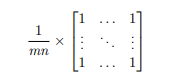
\includegraphics[width=5cm, keepaspectratio]{capitoli/immagini/imgs/filtro-medio.png}
\end{figure}

\subsubsection{Filtro di media ponderata}

\begin{center}
    $g(x,y)=\frac{\sum_{s=-a}^{a}\sum_{t=-b}^{b}w(s,t)f(x+s,y+t)}{\sum_{s=-a}^{a}\sum_{t=-b}^{b}w(s,t)}$
\end{center}

\subsubsection{Filtro Gaussiano}

\begin{figure}[H]
    \centering
    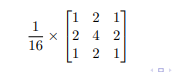
\includegraphics[width=5cm, keepaspectratio]{capitoli/immagini/imgs/filtro-gaussiano.png}
\end{figure}
\textbf{Esempio}
\begin{figure}[H]
    \centering
    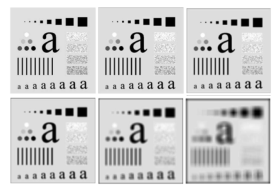
\includegraphics[width=\linewidth, keepaspectratio]{capitoli/immagini/imgs/filtri-l-esempio.png}
\end{figure}

\begin{enumerate}
    \item [a.] Immagine originale di 500 × 500 pixel.
    \item [b.f.] Risultato della sfocatura con filtro medio tramite maschere di
          dimensione 3, 5, 9, 15, 35.
\end{enumerate}
\textbf{Esempio}
\\
Esempio di applicazione del filtro medio
\begin{figure}[H]
    \centering
    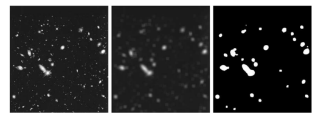
\includegraphics[width=\linewidth, keepaspectratio]{capitoli/immagini/imgs/filtro-l-esempio2.png}
\end{figure}

\begin{enumerate}
    \item [a.] Immagine originale di 528 × 485 pixel.
    \item [b.] Risultato della sfocatura con filtro medio tramite maschera di dimensione 15
    \item [c.]  Risultato dell’applicazione di una soglia.
\end{enumerate}
I rumori non lineari (ad esempio quello impulsivo) non possono essere corretti con i filtri lineari.
Possono essere trattati invece efficacemente con \textbf{filtri non lineari}
\\
\textbf{Esempio:}
\begin{trivlist}
    \item \textbf{Filtro mediano:}  sostituisce al valore di ogni pixel prefissato la
    mediana (valore centrale della lista ordinata) dei
    valori dei pixel nell’intorno fissato.
\end{trivlist}
Il filtro mediano risulta particolarmente adatto a correggere il rumore \textbf{salt and pepper}, a differenza del filtro medio che, come si
vede dall’esempio seguente, non risulta invece particolarmente efficace.

\subsubsection{Esempio: Filtro medio}

\begin{figure}[H]
    \centering
    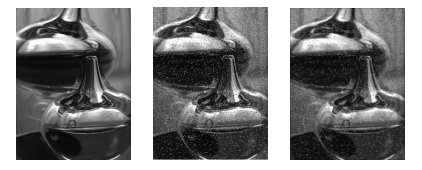
\includegraphics[width=\linewidth, keepaspectratio]{capitoli/immagini/imgs/esempio-filtro-medio.png}
\end{figure}
Immagine originale, immagine corrotta da rumore \textbf{salt and pepper} e
immagine filtrata con \textbf{filtro medio}

\subsubsection{Esempio: Filtro medinao}
\begin{figure}[H]
    \centering
    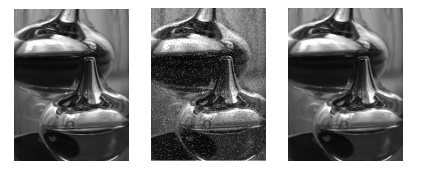
\includegraphics[width=\linewidth, keepaspectratio]{capitoli/immagini/imgs/esempio-filtro-mediano.png}
\end{figure}
Immagine originale, immagine corrotta da rumore \textbf{salt and pepper} e
immagine filtrata con \textbf{filtro mediano}

\subsubsection{Esempio: Filtro medio}
Il \textbf{filtro medio} è invece molto utilizzato ad esempio per correggere il
\textbf{rumore gaussiano.}
\begin{figure}[H]
    \centering
    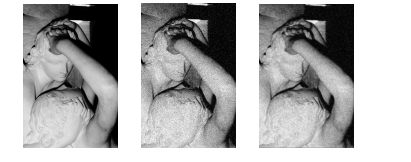
\includegraphics[width=\linewidth, keepaspectratio]{capitoli/immagini/imgs/filtro-medio-esempio2.png}
\end{figure}
Immagine originale, immagine corrotta da rumore gaussiano e immagine filtrata con filtro medio
\subsubsection{Altri filtri (non lineari) basati sulle statistiche d’ordine}
\begin{itemize}
    \item \textbf{Filtro di massimo}
    \item \textbf{Filtro di minimo}
    \item \textbf{Filtro di punto medio}
    \item \textbf{Filtro medio di alpha-trimmed}
\end{itemize}
